% !TeX spellcheck = en-US
% !TeX encoding = utf8
% !TeX program = pdflatex
% !BIB program = biber
% -*- coding:utf-8 mod:LaTeX -*-


% vv  scroll down to line 200 for content  vv


\let\ifdeutsch\iffalse
\let\ifenglisch\iftrue
% EN: This file is loaded before the \documentclass command in the main document

% EN: The following package allows \\ at the title page
%     For more information see https://github.com/latextemplates/scientific-thesis-cover/issues/4
\RequirePackage{kvoptions-patch}

\ifenglisch
  \PassOptionsToClass{numbers=noenddot}{scrbook}
\else
  %()Aus scrguide.pdf - der Dokumentation von KOMA-Script)
  %Nach DUDEN steht in Gliederungen, in denen ausschließlich arabische Ziffern für die Nummerierung
  %verwendet werden, am Ende der Gliederungsnummern kein abschließender Punkt
  %(siehe [DUD96, R3]). Wird hingegen innerhalb der Gliederung auch mit römischen Zahlen
  %oder Groß- oder Kleinbuchstaben gearbeitet, so steht am Ende aller Gliederungsnummern ein
  %abschließender Punkt (siehe [DUD96, R4])
  \PassOptionsToClass{numbers=autoendperiod}{scrbook}
\fi

% Warns about outdated packages and missing caption declarations
% See https://www.ctan.org/pkg/nag
\RequirePackage[l2tabu, orthodox]{nag}

%DE: Neue deutsche Trennmuster
%    Siehe http://www.ctan.org/pkg/dehyph-exptl und http://projekte.dante.de/Trennmuster/WebHome
%    Nur für pdflatex, nicht für lualatex
\RequirePackage{ifluatex}
\ifluatex
  % do not load anything
\else
  \ifdeutsch
    \RequirePackage[ngerman=ngerman-x-latest]{hyphsubst}
  \fi
\fi

\documentclass[
  % fontsize=11pt is the standard
  a4paper,  % Standard format - only KOMAScript uses paper=a4 - https://tex.stackexchange.com/a/61044/9075
  twoside,  % we are optimizing for both screen and two-side printing. So the page numbers will jump, but the content is configured to stay in the middle (by using the geometry package)
  bibliography=totoc,
  %               idxtotoc,   %Index ins Inhaltsverzeichnis
  %               liststotoc, %List of X ins Inhaltsverzeichnis, mit liststotocnumbered werden die Abbildungsverzeichnisse nummeriert
  headsepline,
  cleardoublepage=empty,
  parskip=half,
  %               draft    % um zu sehen, wo noch nachgebessert werden muss - wichtig, da Bindungskorrektur mit drin
  draft=false
]{scrbook}
\usepackage{subfig}

\usetikzlibrary{graphs}

\graphicspath{{../../Simulation/Models/}{./Figs/}}

\renewcommand{\P}{\mathcal{P}}

\newcommand{\A}{\mathcal{A}}
\newcommand{\B}{\mathcal{B}}
\newcommand{\C}{\mathcal{C}}
\newcommand{\D}{\mathcal{D}}

\renewcommand{\L}{\mathcal{L}}
\newcommand{\R}{\mathcal{R}}

\DeclareMathOperator{\AL}{L}
\DeclareMathOperator{\AR}{R}
\DeclareMathOperator{\AW}{W}
\DeclareMathOperator{\AMi}{Mi}
\DeclareMathOperator{\AB}{B}

\newcommand{\BCB}{\xi}

\newcommand{\BranchInterval}{I}
\newcommand{\Branch}{f}

\renewcommand{\O}{\mathcal{O}}
\newcommand{\Cycle}[1]{\O_{#1}}

\newcommand{\F}{\mathcal{F}}



\usepackage[
  title={Is Oil the future?},
  author={Lars K.},
  type=bachelor,
  institute=iaas, % or other institute names - or just a plain string using {Demo\\Demo...}
  course={Medieninformatik},
  examiner={Prof.\ Dr.\ Uwe Fessor},
  supervisor={Dipl.-Inf.\ Roman Tiker,\\Dipl.-Inf.\ Laura Stern,\\Otto Normalverbraucher,\ M.Sc.},
  startdate={July 5, 2018},
  enddate={January 5, 2019}
]{scientific-thesis-cover}

\newacronym{pws}{PWS}{piecewise smooth}


\makeindex

\begin{document}

%tex4ht-Konvertierung verschönern
\iftex4ht
  % tell tex4ht to create picures also for formulas starting with '$'
  % WARNING: a tex4ht run now takes forever!
  \Configure{$}{\PicMath}{\EndPicMath}{}
  %$ % <- syntax highlighting fix for emacs
  \Css{body {text-align:justify;}}

  %conversion of .pdf to .png
  \Configure{graphics*}
  {pdf}
  {\Needs{"convert \csname Gin@base\endcsname.pdf
      \csname Gin@base\endcsname.png"}%
    \Picture[pict]{\csname Gin@base\endcsname.png}%
  }
\fi

%\VerbatimFootnotes %verbatim text in Fußnoten erlauben. Geht normalerweise nicht.

% DE: wird fuer Tabellen benötigt (z.B. >{centering\RBS}p{2.5cm} erzeugt einen zentrierten 2,5cm breiten Absatz in einer Tabelle
\newcommand{\RBS}{\let\\=\tabularnewline}

% EN: To avoid issues with Springer's \mathplus
%     See also http://tex.stackexchange.com/q/212644/9075
\providecommand\mathplus{+}

% DE: typoraphisch richtige Abkürzungen
\newcommand{\zB}{z.\,B.\xspace}
\newcommand{\bzw}{bzw.\xspace}
\newcommand{\usw}{usw.\xspace}
\renewcommand{\dh}{d.\,h.\xspace}

% EN: from hmks makros.tex - \indexify
\newcommand{\toindex}[1]{\index{#1}#1}

% DE: Tipp aus "The Comprehensive LaTeX Symbol List"
\newcommand{\dotcup}{\ensuremath{\,\mathaccent\cdot\cup\,}}

% DE: Anstatt $|x|$ $\abs{x}$ verwenden.
%     Die Betragsstriche skalieren automatisch, falls "x" etwas größer sein sollte...
\newcommand{\abs}[1]{\left\lvert#1\right\rvert}

% DE: für Zitate
\newcommand{\citeS}[2]{\cite[S.~#1]{#2}}
\newcommand{\citeSf}[2]{\cite[S.~#1\,f.]{#2}}
\newcommand{\citeSff}[2]{\cite[S.~#1\,ff.]{#2}}
\newcommand{\vgl}{vgl.\ }
\newcommand{\Vgl}{Vgl.\ }

% EN: For the algorithmic package
\newcommand{\commentchar}{\ensuremath{/\mkern-4mu/}}
\algrenewcommand{\algorithmiccomment}[1]{\hfill $\commentchar$ #1}

% DE: Seitengrößen - Gegen Schusterjungen und Hurenkinder...
\newcommand{\largepage}{\enlargethispage{\baselineskip}}
\newcommand{\shortpage}{\enlargethispage{-\baselineskip}}

\newcommand{\initialism}[1]{%
  \ifdeutsch%
    \textsc{#1}\xspace%
  \else%
    \textlcc{#1}\xspace%
  \fi%
}
\newcommand{\OMG}{\initialism{OMG}}
\newcommand{\BPEL}{\initialism{BPEL}}
\newcommand{\BPMN}{\initialism{BPMN}}
\newcommand{\UML}{\initialism{UML}}

\pagenumbering{arabic}
\Titelblatt

%Eigener Seitenstil fuer die Kurzfassung und das Inhaltsverzeichnis
\deftriplepagestyle{preamble}{}{}{}{}{}{\pagemark}
%Doku zu deftriplepagestyle: scrguide.pdf
\pagestyle{preamble}
\renewcommand*{\chapterpagestyle}{preamble}



%Kurzfassung / abstract
%auch im Stil vom Inhaltsverzeichnis
\ifdeutsch
  \section*{Kurzfassung}
\else
  \section*{Abstract}
\fi

<Short summary of the thesis>

\cleardoublepage


% BEGIN: Verzeichnisse

\iftex4ht
\else
  \microtypesetup{protrusion=false}
\fi

%%%
% Literaturverzeichnis ins TOC mit aufnehmen, aber nur wenn nichts anderes mehr hilft!
% \addcontentsline{toc}{chapter}{Literaturverzeichnis}
%
% oder zB
%\addcontentsline{toc}{section}{Abkürzungsverzeichnis}
%
%%%

%Produce table of contents
%
%In case you have trouble with headings reaching into the page numbers, enable the following three lines.
%Hint by http://golatex.de/inhaltsverzeichnis-schreibt-ueber-rand-t3106.html
%
%\makeatletter
%\renewcommand{\@pnumwidth}{2em}
%\makeatother
%
\tableofcontents

% Bei einem ungünstigen Seitenumbruch im Inhaltsverzeichnis, kann dieser mit
% \addtocontents{toc}{\protect\newpage}
% an der passenden Stelle im Fließtext erzwungen werden.

\listoffigures
\listoftables

%Wird nur bei Verwendung von der lstlisting-Umgebung mit dem "caption"-Parameter benoetigt
%\lstlistoflistings
%ansonsten:
\ifdeutsch
  \listof{Listing}{Verzeichnis der Listings}
\else
  \listof{Listing}{List of Listings}
\fi

%mittels \newfloat wurde die Algorithmus-Gleitumgebung definiert.
%Mit folgendem Befehl werden alle floats dieses Typs ausgegeben
\ifdeutsch
  \listof{Algorithmus}{Verzeichnis der Algorithmen}
\else
  \listof{Algorithmus}{List of Algorithms}
\fi
%\listofalgorithms %Ist nur für Algorithmen, die mittels \begin{algorithm} umschlossen werden, nötig

% Abkürzungsverzeichnis
\printnoidxglossaries

\iftex4ht
\else
  %Optischen Randausgleich und Grauwertkorrektur wieder aktivieren
  \microtypesetup{protrusion=true}
\fi

% END: Verzeichnisse


% Headline and footline
\renewcommand*{\chapterpagestyle}{scrplain}
\pagestyle{scrheadings}
\pagestyle{scrheadings}
\ihead[]{}
\chead[]{}
\ohead[]{\headmark}
\cfoot[]{}
\ofoot[\usekomafont{pagenumber}\thepage]{\usekomafont{pagenumber}\thepage}
\ifoot[]{}


%% vv  scroll down for content  vv %%































%%%%%%%%%%%%%%%%%%%%%%%%%%%%%%%%%%%%%%%%%%%%%%%%%%%%%%%%%%%%%%%%%%%%%%%%%%%%%%
%
% Main content starts here
%
%%%%%%%%%%%%%%%%%%%%%%%%%%%%%%%%%%%%%%%%%%%%%%%%%%%%%%%%%%%%%%%%%%%%%%%%%%%%%%

\only<beamer>{\titleframe}

\begin{frame}{Overview}
	\tableofcontents
\end{frame}

\sectionframe{Recap}
\section{Recap}

\begin{frame}{Complex Model}
	\begin{itemize}
		\item We started with a complex model describing the dynamics of a power converter
		\item It exhibited interesting dynamics we want to understand
		\item Chains of parameter regions with the same period
		      %\item Parameter regions with 2 coexisting cycles in between parameter regions with single cycles
	\end{itemize}
	\vspace{-1em}
	\begin{figure}
		\subfloat[2D period scan]{
			\includegraphics[width=0.3 \textwidth]{99_Yunus/2D_Period_Zoomed/result.png}
		}
		\subfloat[Cobweb at point $A$]{
			\includegraphics[width=0.3 \textwidth]{99_Yunus/Period12/Cobweb_A_12/result.png}
		}
		\subfloat[Cobweb at point $B$]{
			\includegraphics[width=0.3 \textwidth]{99_Yunus/Period12/Cobweb_B2/result.png}
		}
	\end{figure}
\end{frame}

\begin{frame}{Original Model (1/3)}
	\vspace{-2.0em}
	\begin{align}
		\theta      & \mapsto  F(\theta) \mod 2 \pi
		\\
		F(\theta)   & = \begin{cases}
			                F_1(\theta) & \text{if } q \cdot \cos(\theta) > 0 \\
			                F_2(\theta) & \text{if } q \cdot \cos(\theta) < 0
		                \end{cases}
		\\
		F_1(\theta) & = \begin{cases}
			                \theta + z_{L_+} + z_1 & \text{if } z_{L_+} < z_{L_0} \\
			                \theta + z_{L_0} + z_2 & \text{if } z_{L_+} > z_{L_0}
		                \end{cases}
		\\
		F_2(\theta) & = \begin{cases}
			                \theta + z_{R_+} + z_3 & \text{if } z_{R_+} < z_{R_0} \\
			                \theta + z_{R_0} + z_4 & \text{if } z_{R_+} > z_{R_0}
		                \end{cases}
	\end{align}

	\pause
	\vspace{2em}
	This looks ok, but how are these values defined?
	\begin{align*}
		z_1, z_2, z_3, z_4, z_{L_+}, z_{L_-}, z_{R_+}, \text{ and } z_{R_0}
	\end{align*}
\end{frame}

\begin{frame}{Original Model (2/3)}
	The smallest non-negative solutions to the following implicit equations
	\begin{subequations}
		\begin{align}
			(q \cdot \cos(\theta) + \mu \cdot \chi) \cdot e^{\lambda \cdot z_{L_+}}
			 & = q \cdot \cos(\theta + z_{L_+} + z_1) + \mu \cdot \chi \\
			(q \cdot \cos(\theta) + \mu \cdot \chi) \cdot e^{\lambda \cdot z_{L_0}}
			 & = q \cdot \cos(\theta + z_{L_0} + z_1) - \mu \cdot \chi \\
			(q \cdot \cos(\theta) + \mu \cdot \chi) \cdot e^{\lambda \cdot z_{R_+}}
			 & = q \cdot \cos(\theta + z_{R_+} + z_1) + \mu \cdot \chi \\
			(q \cdot \cos(\theta) + \mu \cdot \chi) \cdot e^{\lambda \cdot z_{R_0}}
			 & = q \cdot \cos(\theta + z_{R_0} + z_1) - \mu \cdot \chi
		\end{align}
	\end{subequations}
	\vspace{-2em}
	\begin{subequations}
		\begin{align}
			(q \cdot \cos(\theta + z_{L_+}) + \chi + 1) \cdot e^{\lambda \cdot z_1} - 1
			 & = q \cdot  \cos(\theta + z_{L_+} + z_1) + \mu \cdot \chi \\
			(q \cdot \cos(\theta + z_{L_0}) + \chi + 1) \cdot e^{\lambda \cdot z_2} + 1
			 & = q \cdot  \cos(\theta + z_{L_0} + z_2) - \mu \cdot \chi \\
			(q \cdot \cos(\theta + z_{R_+}) + \chi + 1) \cdot e^{\lambda \cdot z_3} - 1
			 & = q \cdot  \cos(\theta + z_{L_+} + z_3) + \mu \cdot \chi \\
			(q \cdot \cos(\theta + z_{R_0}) + \chi + 1) \cdot e^{\lambda \cdot z_4} + 1
			 & = q \cdot  \cos(\theta + z_{R_0} + z_4) - \mu \cdot \chi
		\end{align}
	\end{subequations}
\end{frame}

\begin{frame}{Original Model (3/3)}
	\vspace{-3.0em}
	\begin{align}
		\chi    & = \dfrac{R \cdot \chi_0}{\beta \cdot E_0} \\
		\lambda & = \dfrac{-R}{L \cdot 2 \cdot \pi \cdot f} \\
		q       & = \dfrac{R \cdot V_m}{\beta \cdot E_0}
	\end{align}

	Normalized and varied Parameters:
	\begin{align*}
		E_0, \chi_0
	\end{align*}

	Symmetry in this model:
	\begin{align}
		F(\theta + \pi) = F(\theta) + \pi \mod 2 \pi
	\end{align}

	\begin{flushright}
		Definition and symmetry from \cite{akyuz2022}
	\end{flushright}
\end{frame}

\begin{frame}{Minimal Reproducing Model Dynamics}
	\vspace{-1em}
	\begin{figure}
		\subfloat[Original]{
			\includegraphics[width=0.3 \textwidth]{99_Yunus/2D_Period_Zoomed/result.png}
		}
		\qquad
		\subfloat[Our new model]{
			\includegraphics[width=0.3 \textwidth]{60_MinimalRepr/2D_Period_Whole_noPoints/result.png}
		}
	\end{figure}
	With this simpler model, we explained the structures
\end{frame}

\begin{frame}{Definition of the Minimal Reproducing Model (1/2)}
	\vspace{-3.0em}
	\begin{align}
		x \mapsto f(x) \mod 1
	\end{align}

	\begin{align}
		f(x) & = \begin{cases}
			         g(x)                                        & \text{ if } x < \frac{1}{2} \\
			         g\left(x - \frac{1}{2}\right) + \frac{1}{2} & \text{ else}
		         \end{cases}
	\end{align}

	\begin{align}
		g(x) & = \begin{cases}
			         l(x) = a_L \cdot x^2 + b_L \cdot x + c_L & \text{ if } x < \frac{1}{4} \\
			         r(x) = b_R \cdot x + c_R                 & \text{ else}
		         \end{cases}
	\end{align}
\end{frame}

\begin{frame}{Definition of the Minimal Reproducing Model (2/2)}
	\vspace{-1em}
	\begin{columns}
		\begin{column}{.7 \textwidth}
			Fixed parameters:
			\begin{align*}
				a_L = 4, b_L = -\frac{1}{2}
			\end{align*}

			Variable parameters
			\begin{align*}
				 & c_L, b_R, c_R                                                    \\
				\text{where} \qquad
				 & c_L = p_y,                                                       \\
				 & b_R = 4 \cdot (B - A), c_R = 2A - B                              \\
				\text {and} \qquad
				 & A = p_x, \text{and } B = \frac{1}{2} + \epsilon \text{ is fixed}
			\end{align*}

			$A$ and $B$ are intermediated parameters for modeling the values of the left ($A$) and right ($B$) borders of $r(x)$
		\end{column}
		\begin{column}{.3 \textwidth}
			\begin{figure}
				\centering
				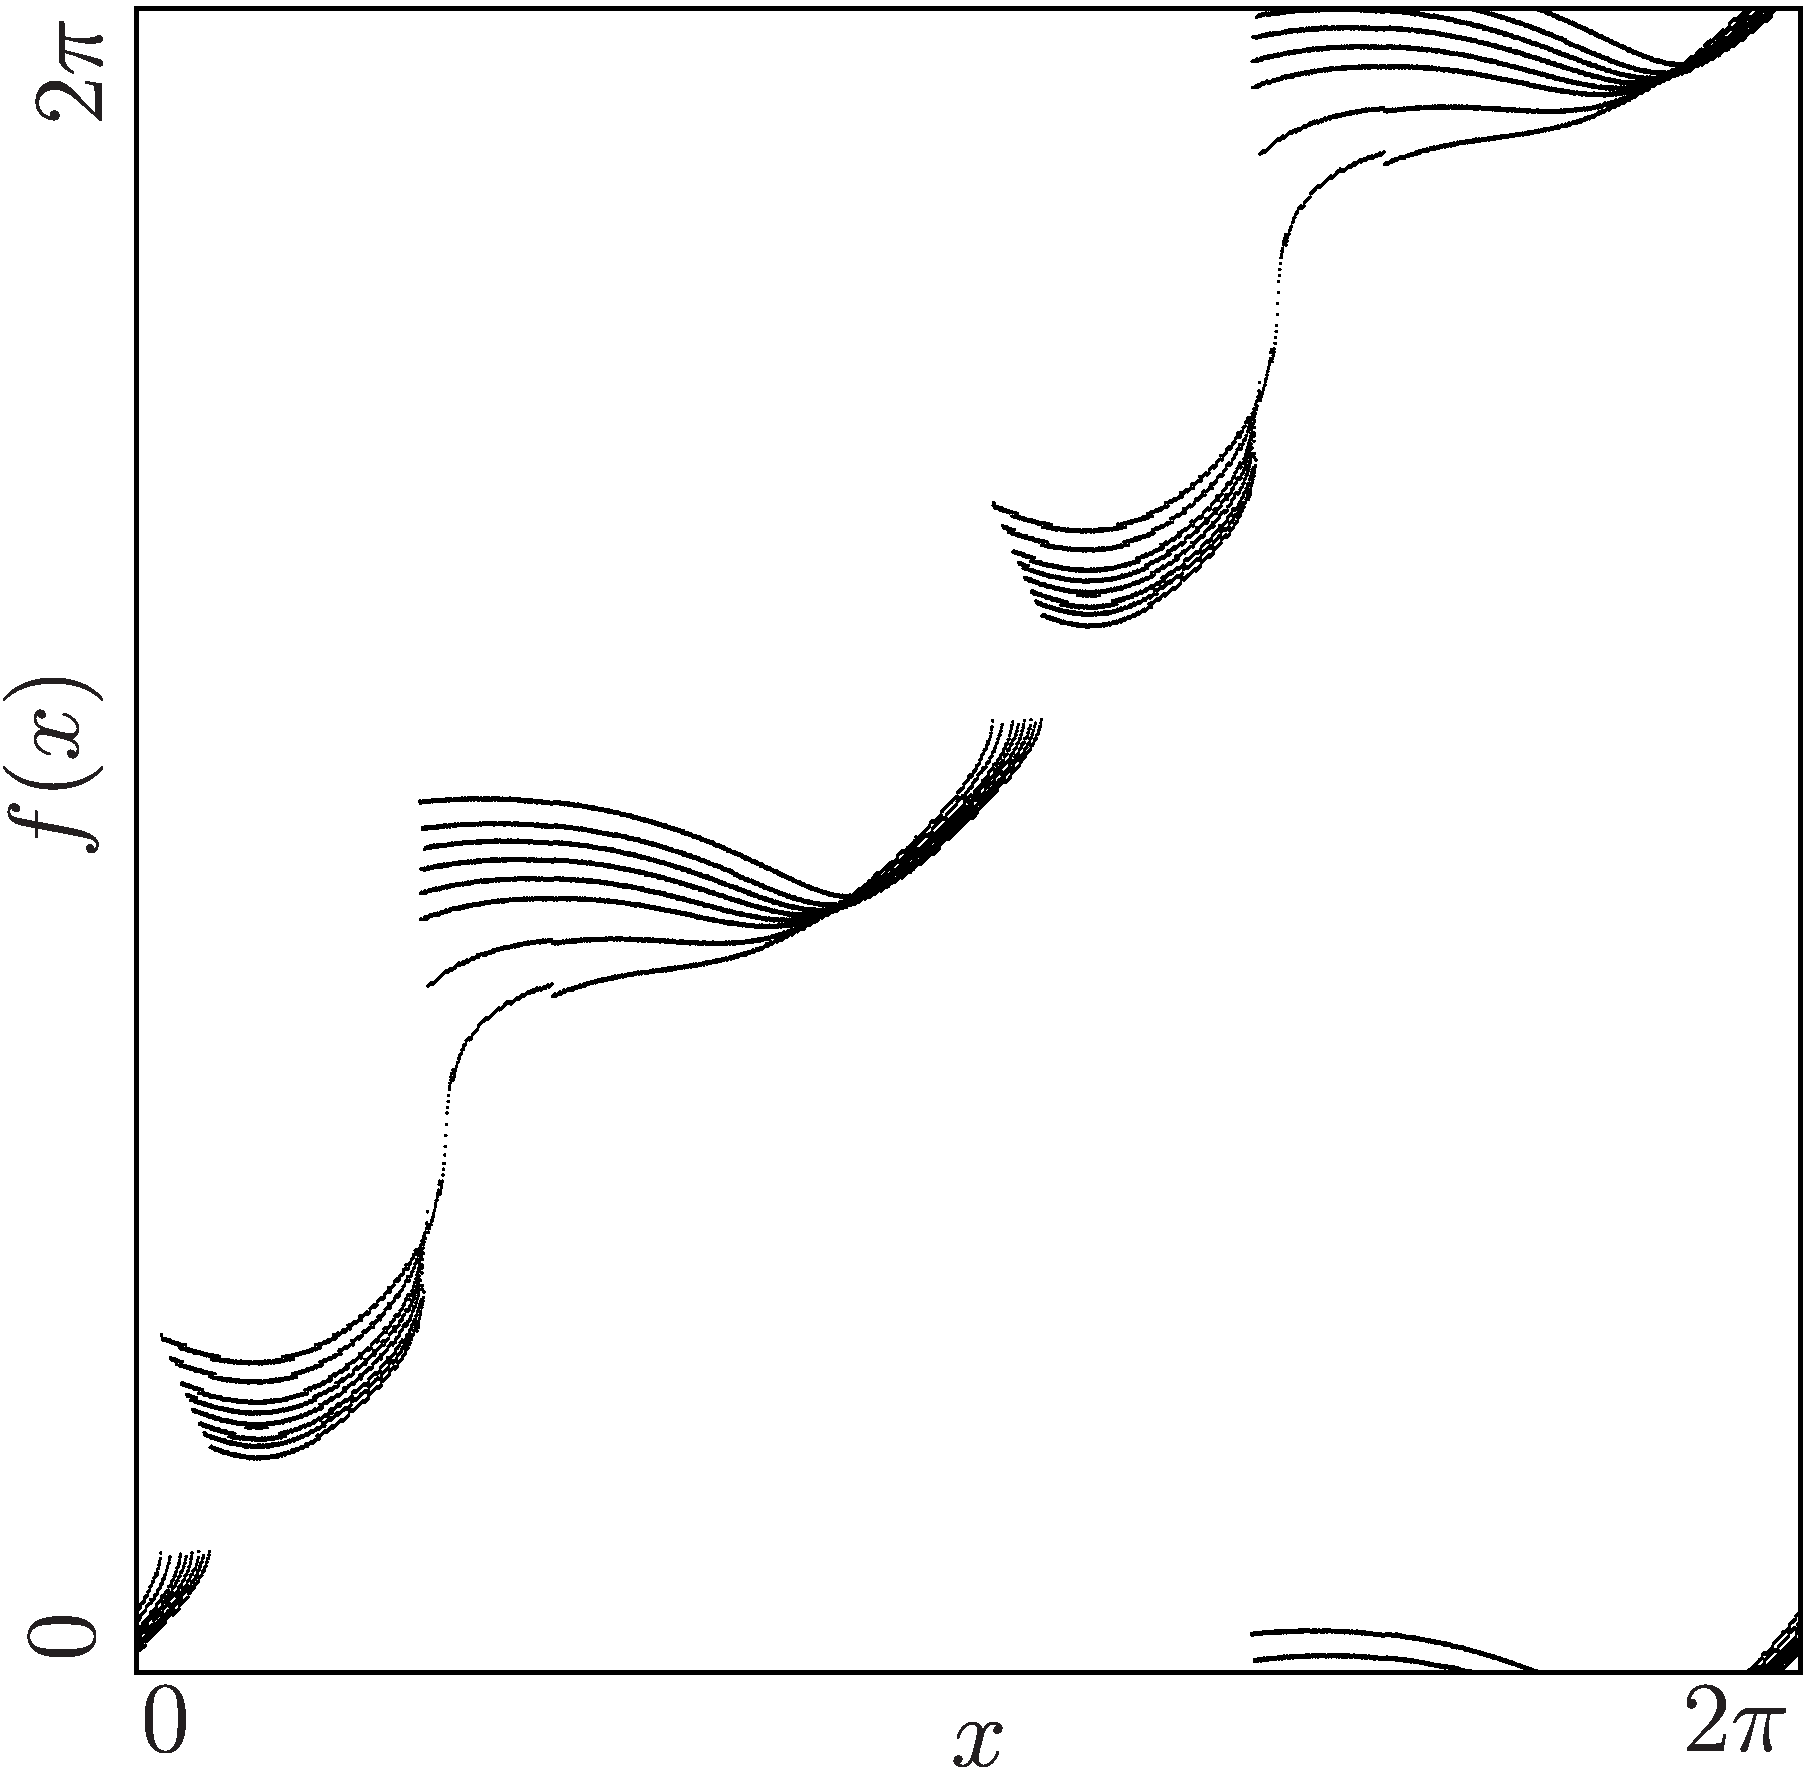
\includegraphics[height=.5 \textheight]{60_MinimalRepr/ParameterEffects/AB/illustration.png}
				\caption*{Illustration of the parameters $A$ and $B$}
			\end{figure}
		\end{column}
	\end{columns}
\end{frame}

\begin{frame}{The Next Step}
	Research question 3 remaining: What else can happen?

	\pause
	\vspace{2em}
	Hypothesis: Period Adding
	\begin{itemize}
		\item This is typical for models of power converters
		\item This is typical for discontinuous models
		\item This is typical in between such chains of the same period
	\end{itemize}
\end{frame}

\begin{frame}{Symbolic Sequences}
	Cycles are described using symbolic sequences.
	Sequence of symbols, indicating on which partition of the function the points of the cycle are.
	\vspace{.5em}
	\begin{columns}
		\hspace{5em}
		\begin{column}{.3 \textwidth}
			\begin{figure}
				\includegraphics[width=\textwidth]{60_MinimalRepr/Cobweb_E16/result.png}
			\end{figure}
		\end{column}
		\hspace{3em}
		\begin{column}{.6 \textwidth}
			\begin{itemize}
				\item Our minimal model
				\item Cycle of period 16
				\item Symbolic Sequence: $\A^5\B^3\C^5\D^3$
			\end{itemize}
		\end{column}
	\end{columns}
\end{frame}

\sectionframe{What is Period-adding?}
\section{What is Period-adding?}

\begin{frame}{Farey Sequences}
    \begin{definition}
        $\F^m$
    \end{definition}
    \todo{Definition of Farey Sequences $\F^m$}
    \begin{theorem}
        $\dfrac{a_1}{b_1}$
    \end{theorem}
    \todo{Theorem of Farey Addition}
    \todo{overlay: tree}
\end{frame}

\begin{frame}{Farey-trees with Symbolic Sequences}
    \begin{itemize}
        \item Keep the structure of the tree
        \item Replace starting nodes with symbolic sequences
        \item Use concatenation instead of Farey-addition $\oplus$
    \end{itemize}
    \todo{overlay: tree with L and R symbolic sequences}
\end{frame}

\begin{frame}{Rotation Numbers}
    \begin{definition}
        $\dfrac{|\sigma|_L}{|\sigma|}$
    \end{definition}
    \todo{define rotation numbers for systems w 2 symbols}
    \begin{theorem}
        Concatenation of two cycles is Farey-addition of their rotation numbers
    \end{theorem}
    \todo{complete theorem}
    So we can replace the symbolic sequences in the last tree with their rotation numbers and will get a valid Farey-tree.
    \todo{overlay: tree}
\end{frame}

\begin{frame}{Period-adding}
    \todo{example with graphs: bifurcation, period \\ from L08 p15}
    \todo{chain example from simpson thesis}
\end{frame}
\sectionframe{Period-adding-like Structures in the Archetypal Model}
\section{Period-adding-like}

\begin{frame}{Parameter Changes Needed}
	\vspace{-1em}
	\begin{figure}
		\includegraphics[width=.3 \textwidth]{60_MinimalRepr/Cobweb_E16/result.png}
		\quad
		\includegraphics[width=.3 \textwidth]{62_MinimalRepr_Adding/Cob_1_ZCorn/result.png}
	\end{figure}
	\vspace{1em}
	Got rid of the local minima on branches $f_\A$ and $f_\C$
\end{frame}

\begin{frame}{Period-adding-like Structures in the Archetypal Model}
	\begin{figure}
		\includegraphics[width=.4 \textwidth]{62_MinimalRepr_Adding/2D_Regions_1/Manual/result.png}
		\quad
		\includegraphics[width=.4 \textwidth]{62_MinimalRepr_Adding/2D_Period_add_zoom/result.png}
	\end{figure}
\end{frame}

\begin{frame}{Changes to the Bifurcation Structure}
	\begin{itemize}
		\item ``Type B'' parameter regions disappeared
		\item ``Type A'' parameter regions of the same chains start overlapping
		      \pause
		\item New space in-between chains
	\end{itemize}
\end{frame}

\begin{frame}{Describing the Period-adding-like Structures}
	\vspace{-1em}
	\begin{figure}
		\only<1>{
			\includegraphics[width=.4 \textwidth]{62_MinimalRepr_Adding/2D_Period_add_zoom_hor/result.png}
			\qquad
			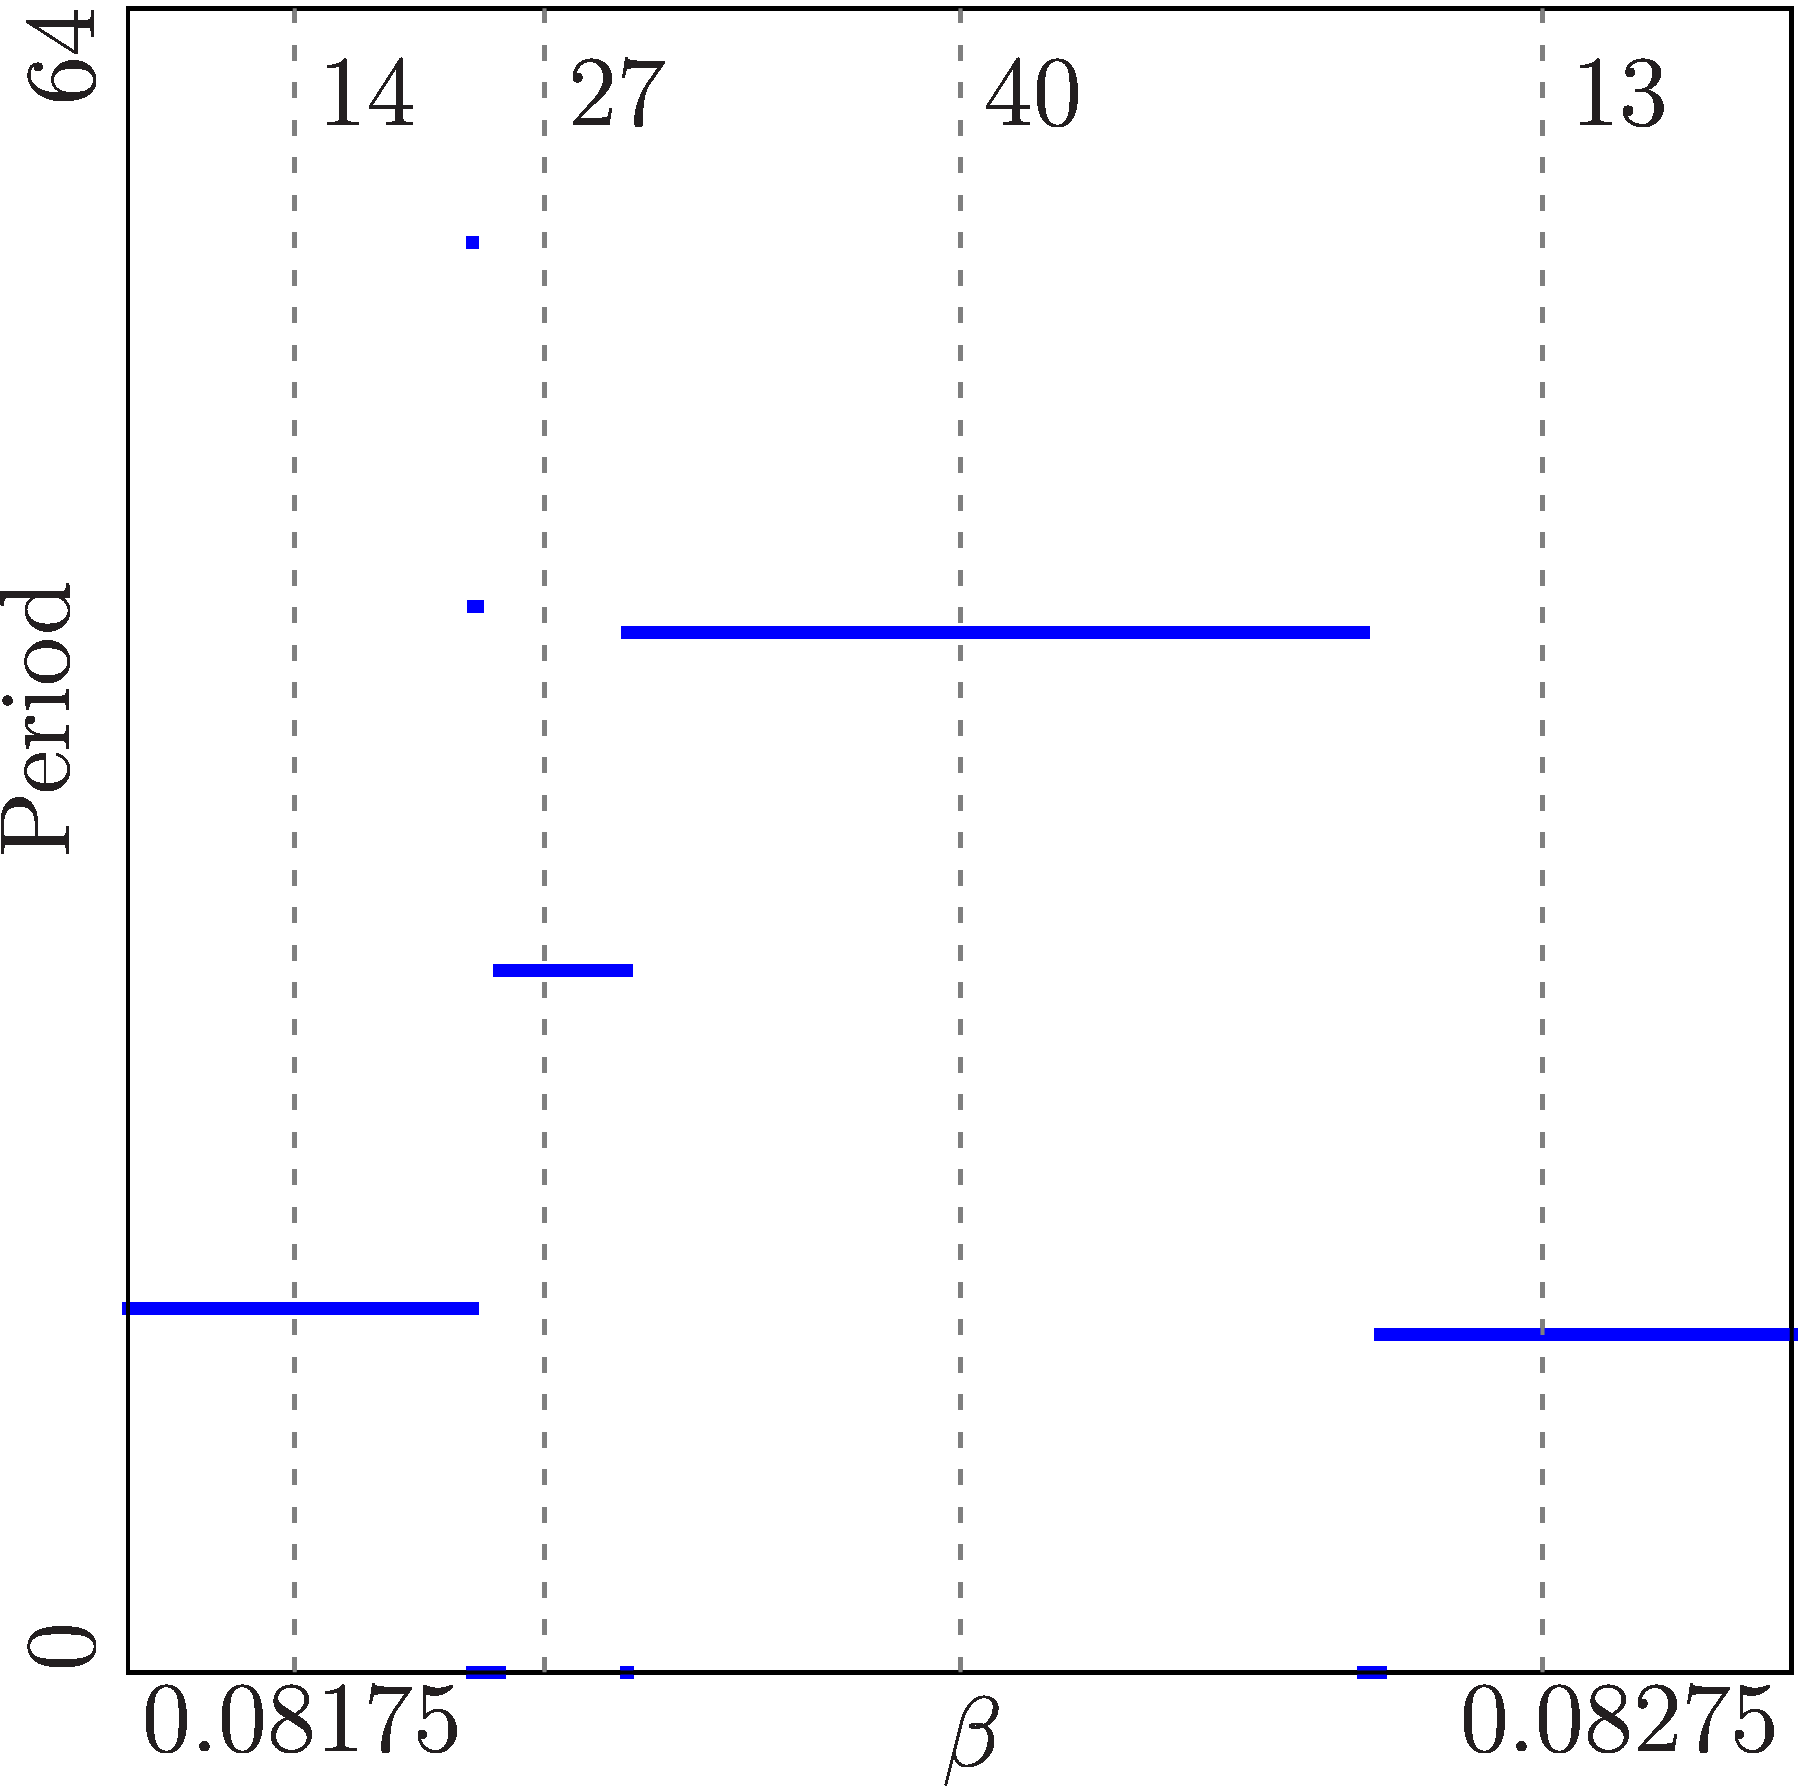
\includegraphics[width=.4 \textwidth]{../Figures/7/7.12b/result.png}
			%			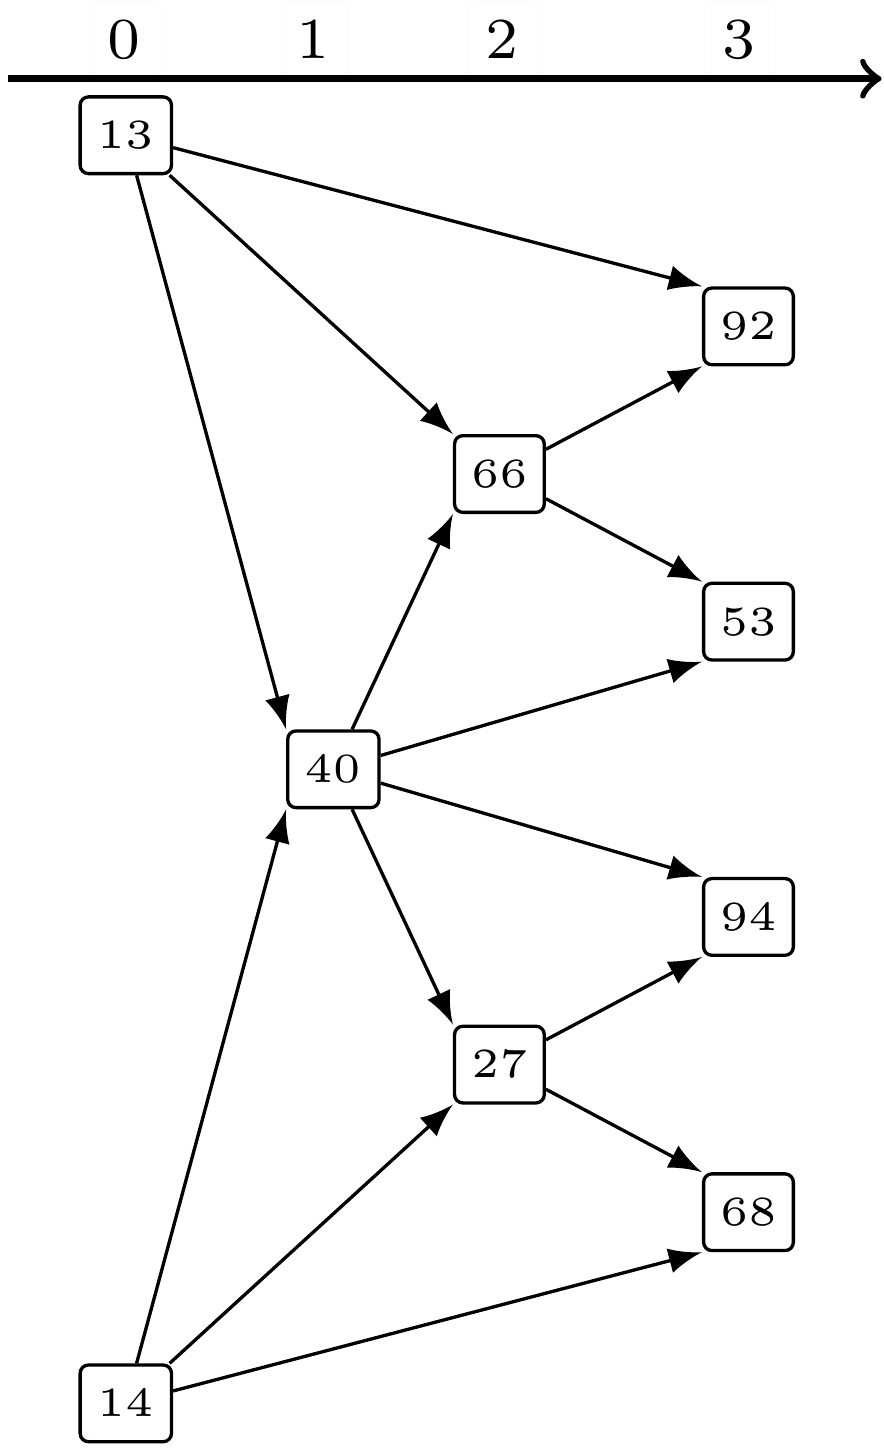
\includegraphics[width=.25 \textwidth]{../../Report/Figures/FareyTrees/Minrep_Adding_larger_Full_Period_3/adding.png}
		}
		\only<2>{
			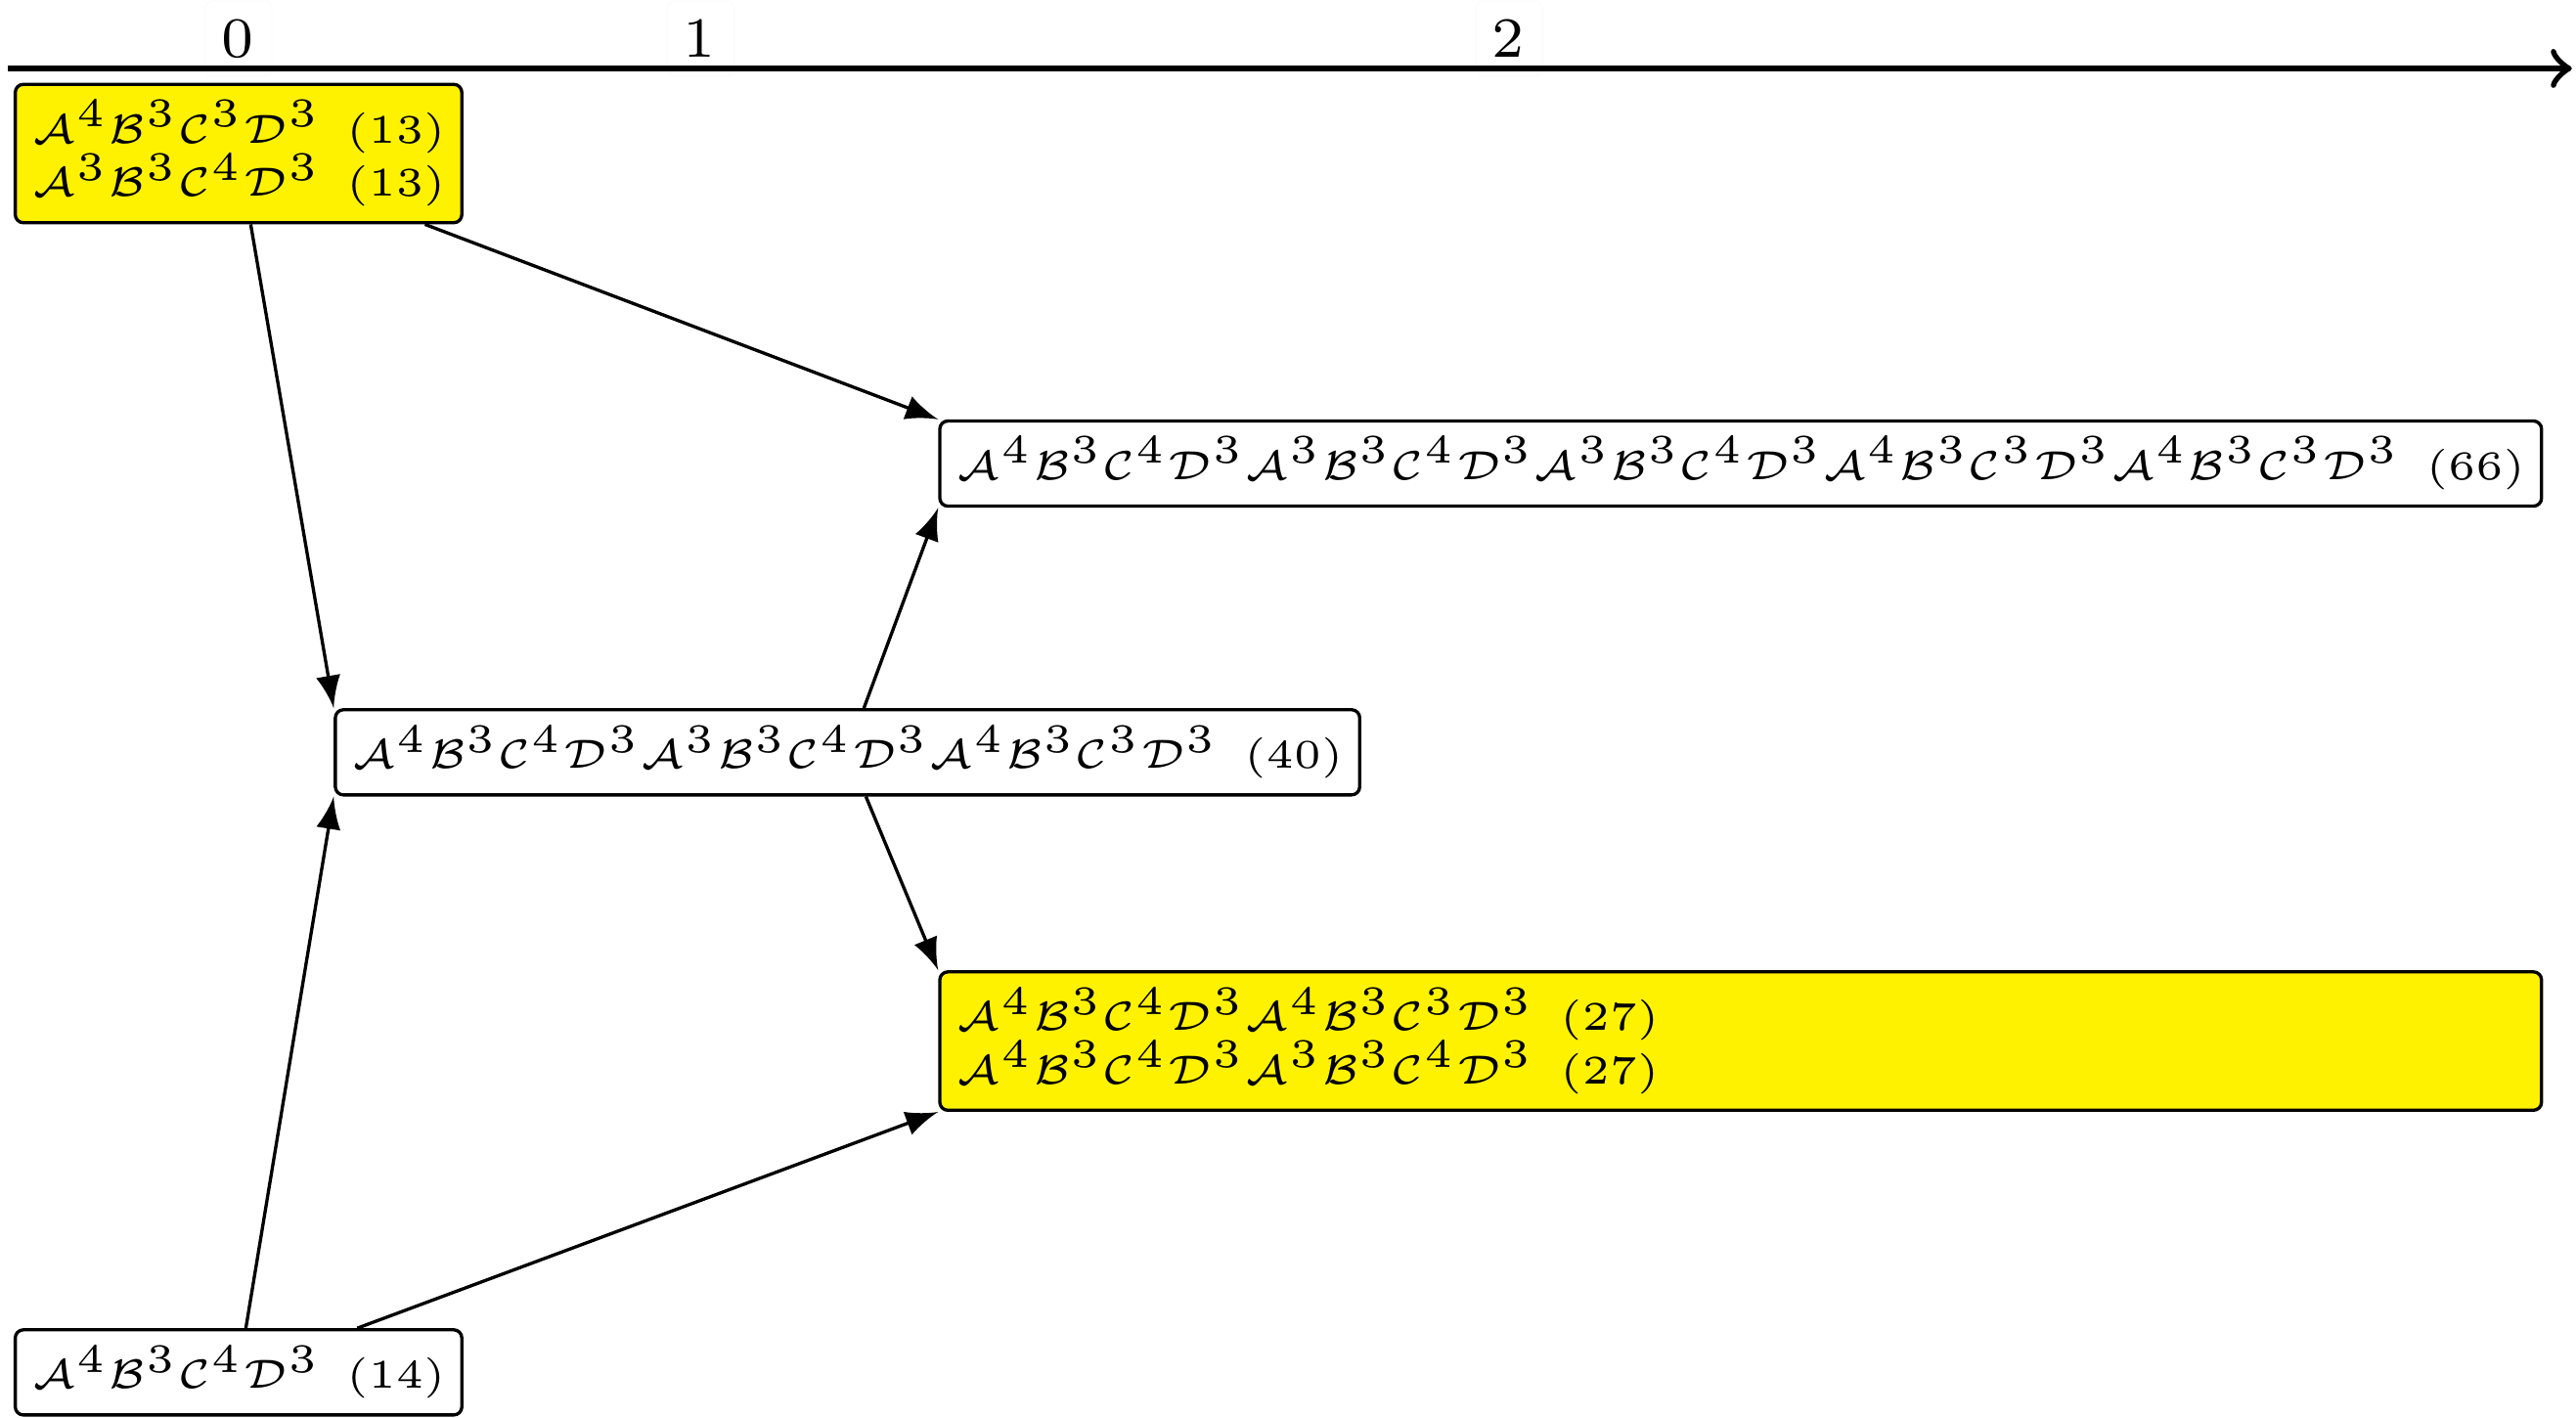
\includegraphics[width=.7 \textwidth]{../Figures/7/7.13/adding.png}
		}
	\end{figure}
\end{frame}

\begin{frame}{Problems with the Period-adding-like Structures}
	This is not period-adding
	\pause
	\begin{itemize}
		\item Periods don't add \pause
		\item Symbolic sequences don't concatenate
	\end{itemize}
\end{frame}

\sectionframe{The Halved Archetypal Model}
\section{Halved}

\begin{frame}{Lifting the Model}
	\vspace{-1em}
	\begin{columns}
		\begin{column}{.4 \textwidth}
			\begin{figure}
				\includegraphics[width=\textwidth]{63_MinimalRepr_Adding_Halved/Cob_Vis_s/Manual/result.png}
			\end{figure}
		\end{column}
		\begin{column}{.5 \textwidth}
			\pause
			\begin{itemize}
				\item Lift the model from $[0, 1)$ to $\mathbb{R}$ \pause
				\item The lifted model repeats every $1$ step \pause
				\item But it even repeats every $\frac{1}{2}$ step because of the built-in symmetry \pause
				\item Drop the model to $[0, \frac{1}{2})$ \pause
			\end{itemize}
			\begin{align*}
				x    & \mapsto g(x) \mod \frac{1}{2}                                              \\
				g(x) & = \begin{cases}
					         g_L(x) = a_L \cdot x^2 + b_L \cdot x + c_L & \text{ if } x < \frac{1}{4} \\
					         g_R(x) = b_R \cdot x + c_R                 & \text{ else}
				         \end{cases}
			\end{align*}
		\end{column}
	\end{columns}
\end{frame}

\begin{frame}{Period-adding in the Halved Archetypal Model (1/2)}
	\vspace{-1em}
	\begin{figure}
		\only<1>{
			\includegraphics[width=.4 \textwidth]{63_MinimalRepr_Adding_Halved/2D_Period_add_zoom_hor/result.png}
			\quad
			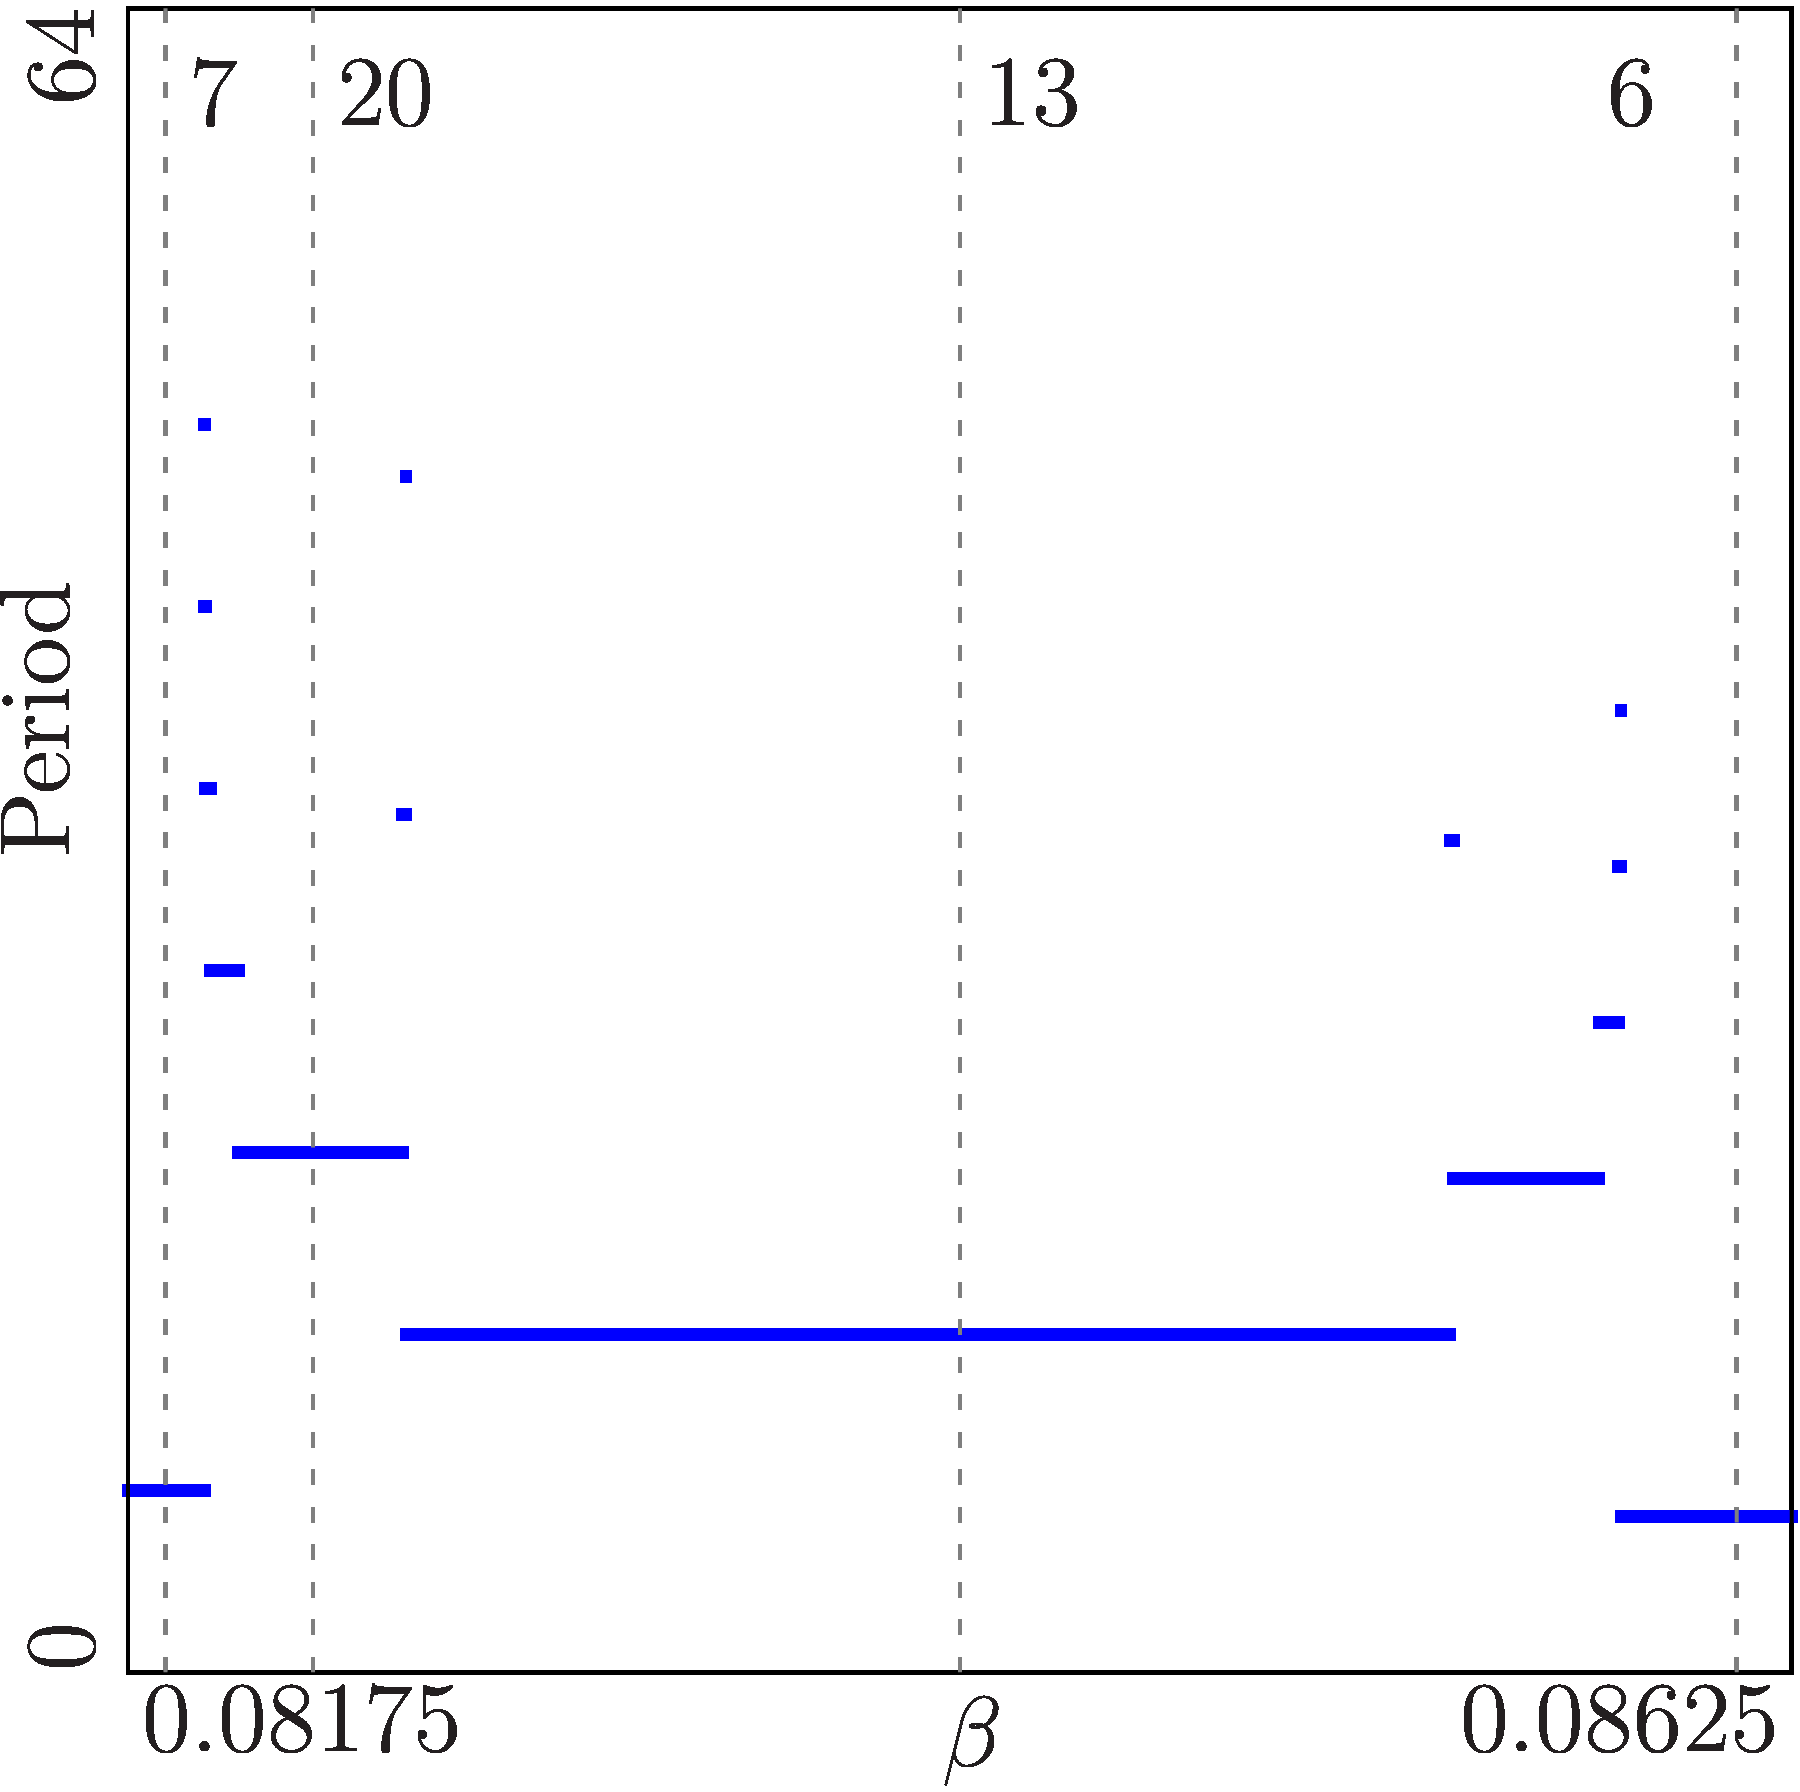
\includegraphics[width=.4 \textwidth]{../Figures/7/7.19b/result.png}
		}
		\only<2>{
			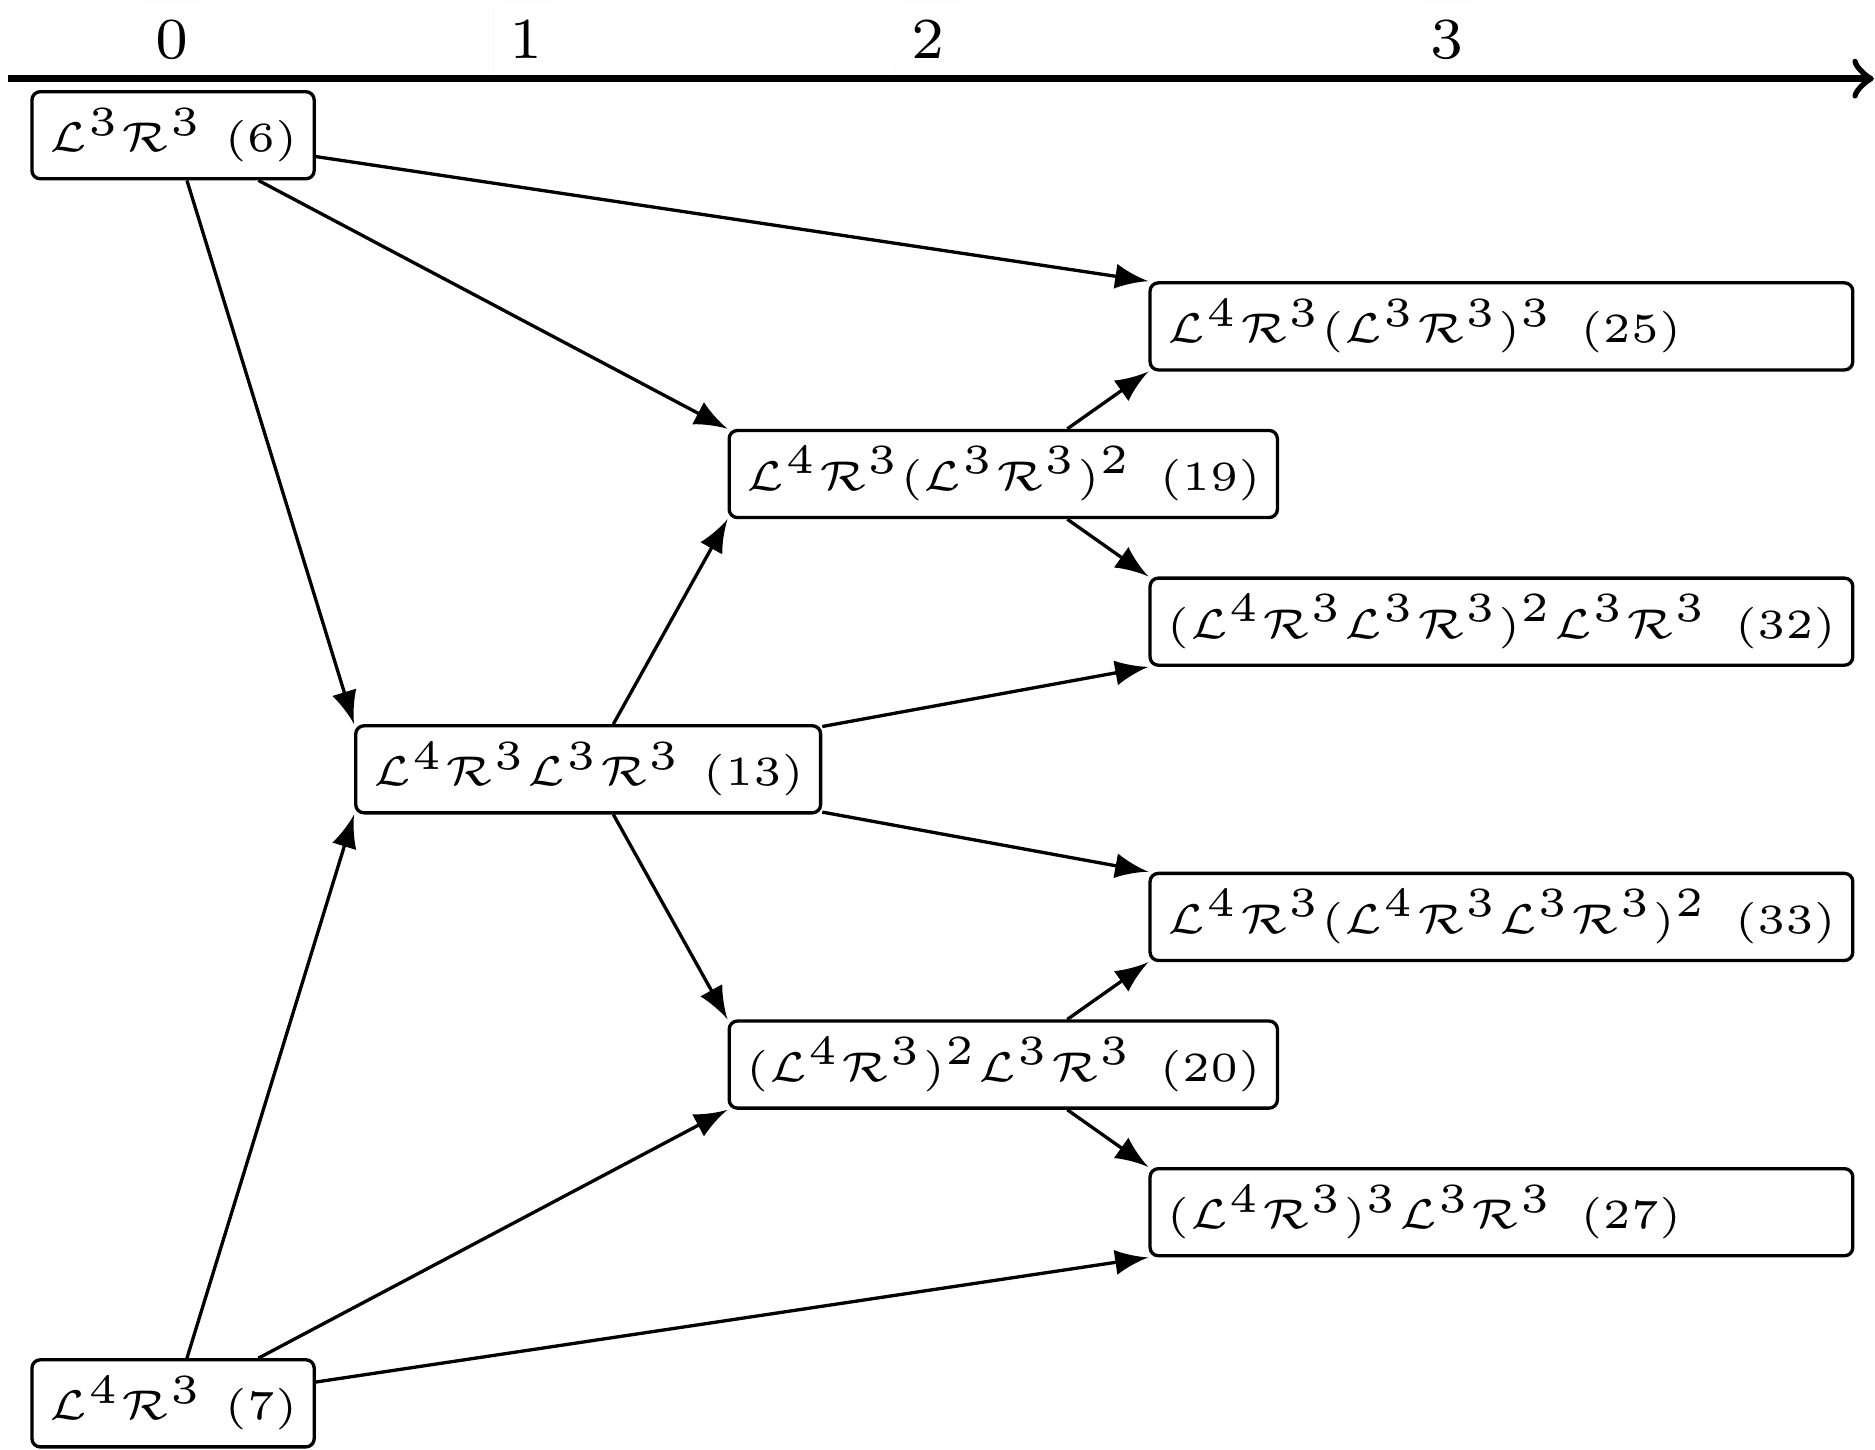
\includegraphics[width=.6 \textwidth]{../Figures/7/7.20/adding.png}
		}
	\end{figure}
\end{frame}

\begin{frame}{Period-adding in the Halved Archetypal Model (2/2)}
	This is period-adding
	\begin{itemize}
		\item Periods add up
		\item Symbolic sequences concatenate
	\end{itemize}
	\pause
	\vspace{1em}
	\begin{center}
		\begin{tikzpicture}
			\node (FC) at (0, 1) {Cycles in Full Model};
			\node (FB) at (6, 1) {Bifurcation Structure};

			\node (HC) at (0, 0) {Cycles in Halved Model};
			\node (HA) at (6, 0) {Period-adding};

			\draw[->] (FC) -- (HC);
			\draw[->] (HC) -- (HA) node[midway,above] {\tiny explained};
			\draw[->] (HA) -- (FB);
			\draw[->] (FC) -- (FB) node[midway,above] {\tiny ???};
		\end{tikzpicture}
	\end{center}
\end{frame}

\begin{frame}{Some Definitions}
	\vspace{-1em}
	\begin{definition}[Syllables]
		A syllable is a subsequence of maximal length consisting of only one symbol. \\[1em]
		A 2-syllable is a pair of syllables next to each other.
		A 4-syllable is a quadrupel of syllables next to each other.
	\end{definition}
	\pause
	Example: $\L^4\R^3\L^3\R^3$ has the syllables $\L^4$, $\L^3$, and $\R^3$ twice.
	\vspace{1em}
	\begin{itemize}
		\pause
		\item One rotation in the halved model corresponds to one 2-syllable
		\item One rotation in the full model corresponds to one 4-syllable
	\end{itemize}
\end{frame}

\begin{frame}{Translating Symbolic Sequences (1/2)}
	\vspace{-1em}
	\begin{definition}[Translating 4-syllables]
		The function $t$ translates one 4-syllable from the halved model to one 4-syllable in the full model.
		\begin{align*}
			t: \L^a\R^b\L^c\R^d \mapsto \A^a\B^b\C^c\D^d
		\end{align*}
	\end{definition}

	\pause
	From the ad-hoc method:
	\begin{itemize}
		\item We can only translate 4-syllables (two rotations in the halved model) at a time
		\item Especially: We cannot translate a 2-syllable alone
	\end{itemize}
	\pause
	\vspace{1em}
	Number of 2-syllables is odd in the halved model $\Rightarrow$ Wrap around once
\end{frame}

\begin{frame}{Translating Symbolic Sequences (2/2)}
	\begin{itemize}
		\item Start at every 2-syllable of the original symbolic sequence
		\item Omit equivalent resulting symbolic sequences
		      \pause \vspace{2em}
		\item Only the first two 2-syllables matter
		\item Number of 2-syllables is odd $\Rightarrow$ Both results are equivalent
	\end{itemize}
\end{frame}

\begin{frame}{The First Consequences}
	\vspace{3em}
	\begin{theorem}[Periods and Coexistence in the Full Model]
		An $n$-cycle in the halved model manifests as
		\begin{itemize}
			\item a single $2n$-cycle in the full model if it has an odd number of 2-syllables
			\item two coexisting $n$-cycles in the full model if it has an even number of 2-syllables
		\end{itemize}
	\end{theorem}
	%	\pause
	%	Examples:
	%	\begin{itemize}
	%		\item $\L^4\R^3$ (Period 7) manifests as a single cycle $\A^4\B^3\C^4\D^3$ (Period 14)
	%		\item $\L^4\R^3\L^3\R^3$ (Period 13) manifests as two cycles
	%		      \begin{itemize}
	%			      \item $\A^4\B^3\C^3\D^3$ (Period 13) and
	%			      \item $\A^3\B^3\C^4\D^3$ (Period 13)
	%		      \end{itemize}
	%	\end{itemize}
\end{frame}

\begin{frame}{The First Consequences}
	\vspace{2em}
	\begin{theorem}[Coexistence in Child Nodes]
		A node in the Farey-tree is associated
		\begin{itemize}
			\item with a single cycle if
			      \begin{itemize}
				      \item one parent node is associated with 2 coexisting cycles and the other parent node is associated with a single cycle.
			      \end{itemize}
			      \pause
			\item with two coexisting cycles if
			      \begin{itemize}
				      \item both parent nodes are associated with single cycles, or
				      \item both parent nodes are associated with two coexisting cycles each.
			      \end{itemize}
		\end{itemize}
	\end{theorem}
	\pause
	\vspace{1em}
	The third case does not appear in our adding structures (proven in report)
	\begin{tikzpicture}[remember picture,overlay]
		\node[xshift=-11em,yshift=-7.1em] at (current page.north east) {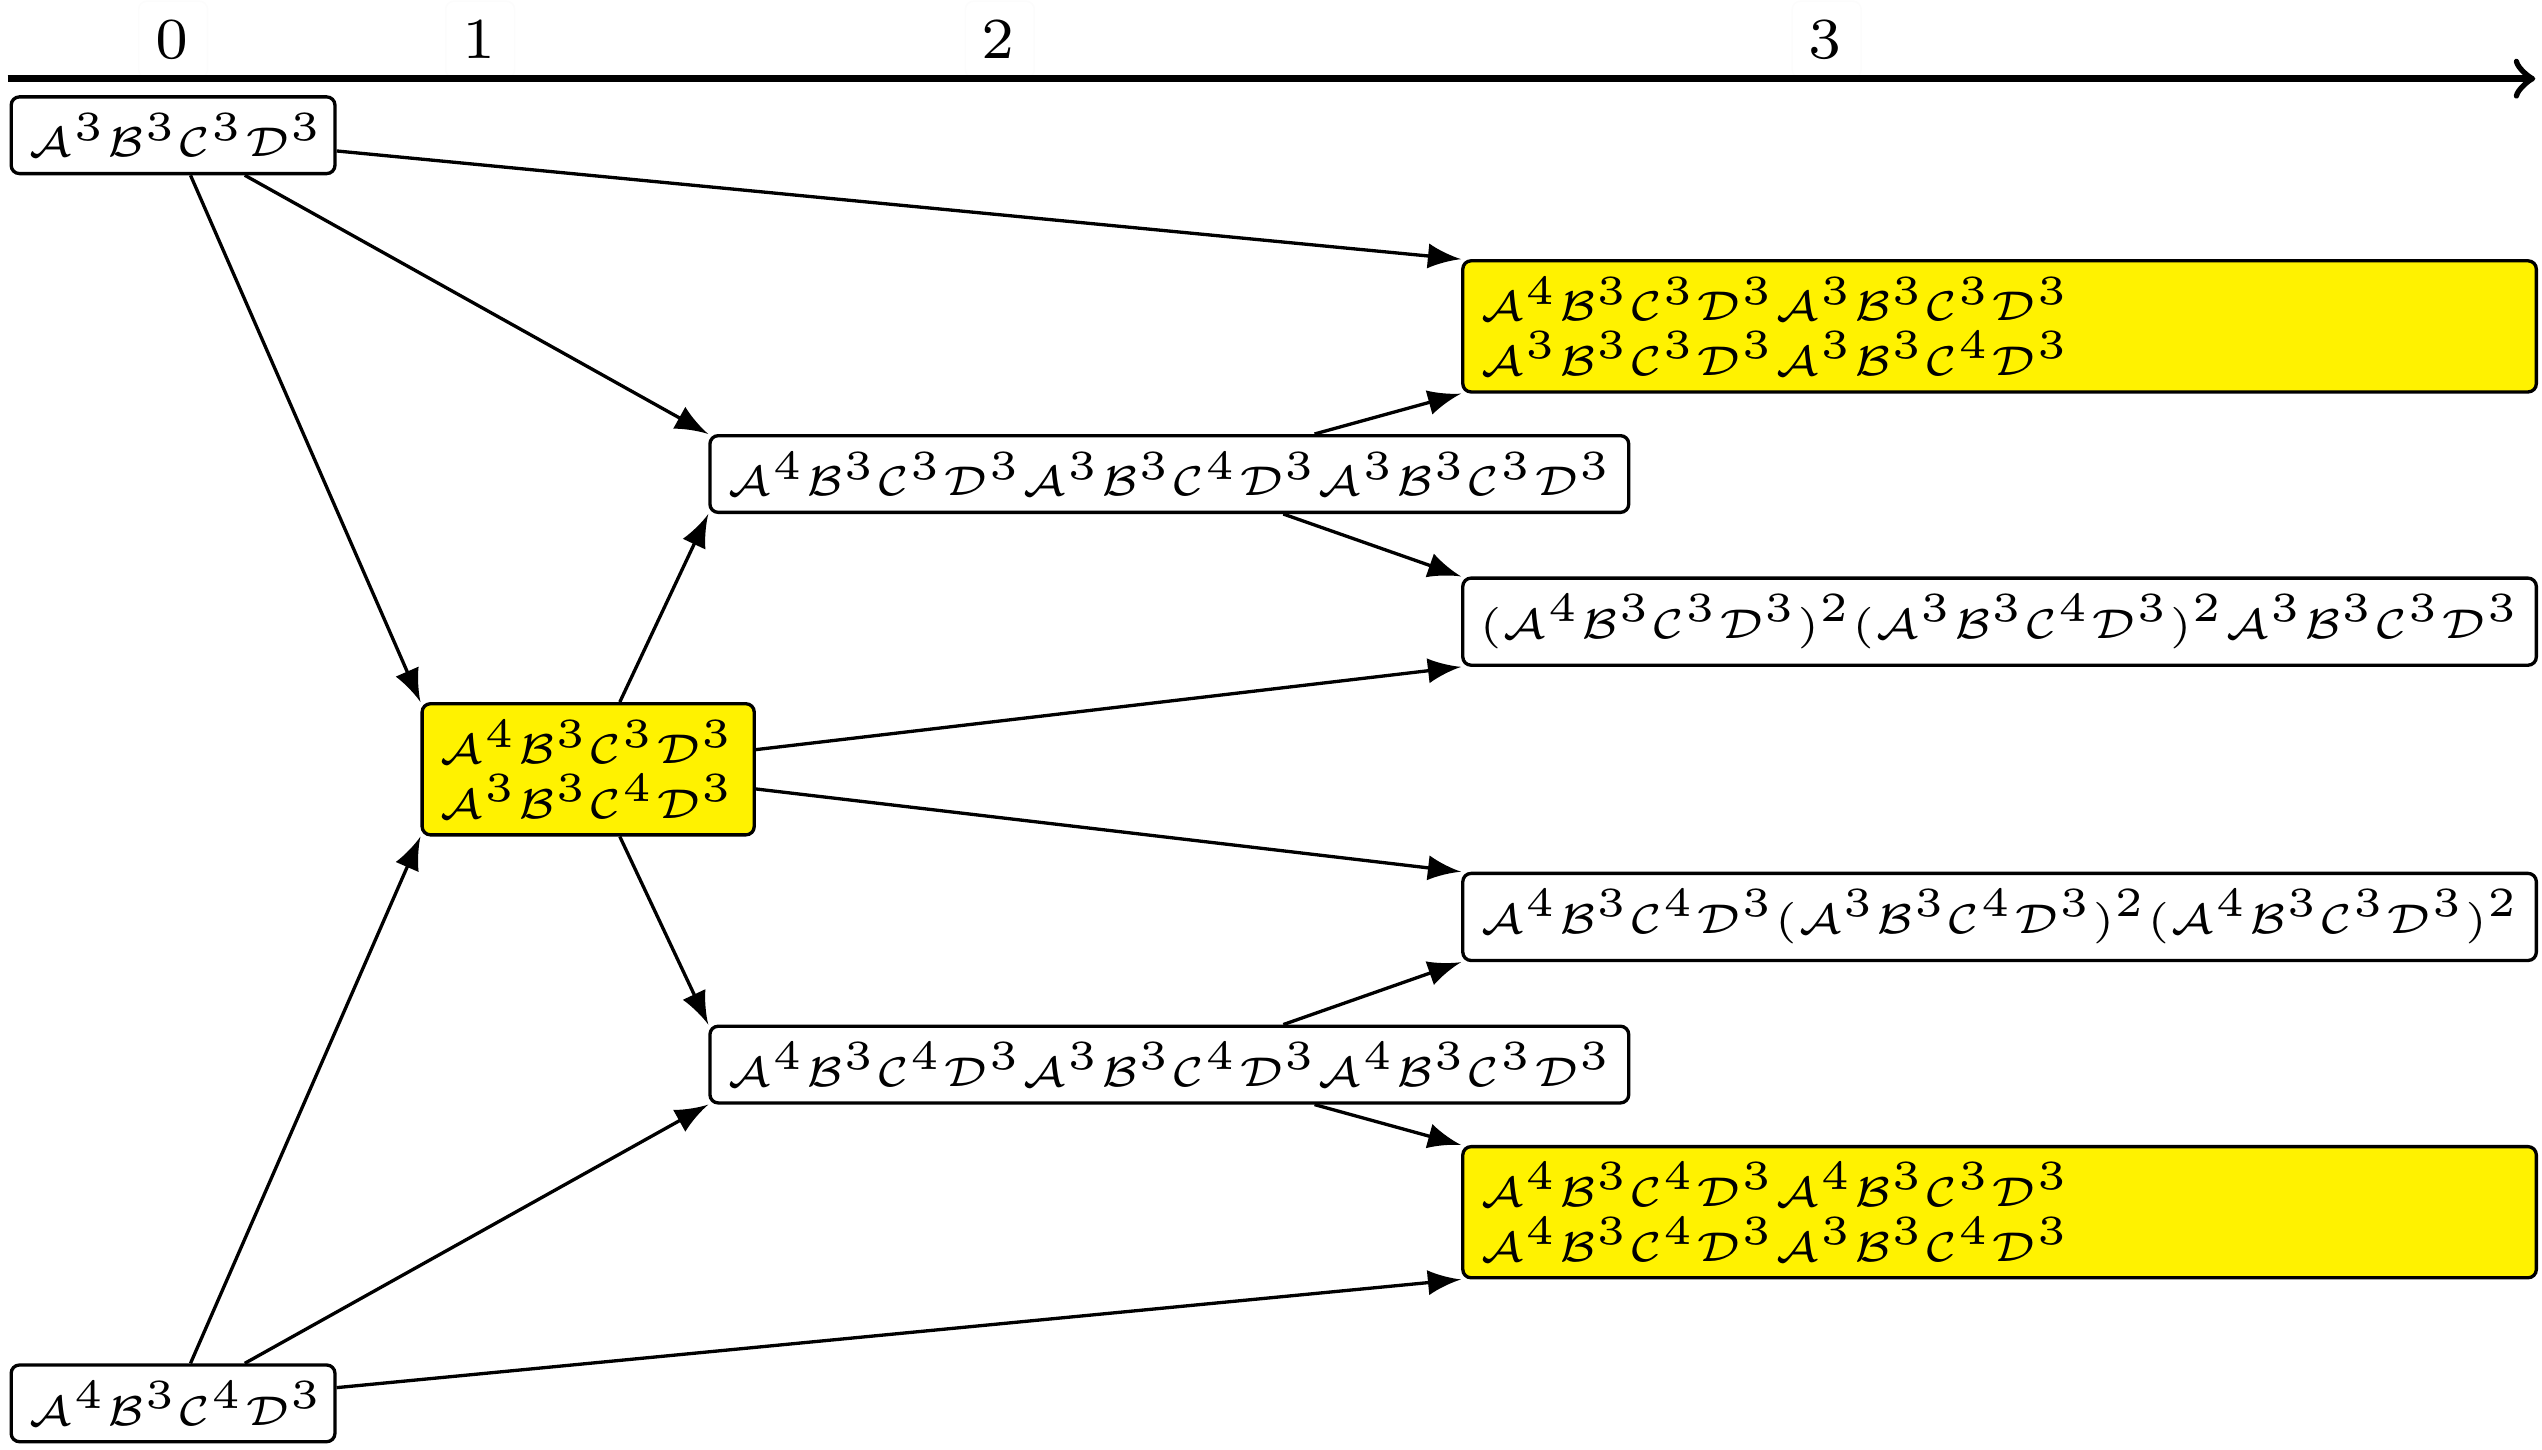
\includegraphics[height=.5 \textheight]{../../Report/Figures/FareyTrees/Minrep_Adding_larger_Full_3/adding.png}};
	\end{tikzpicture}
\end{frame}

\begin{frame}{Explanation of the Period-adding-like Structures}
	\begin{itemize}
		\item Unusual bifurcation structures similar to period-adding structures
		      \pause
		\item Idea: Halved archetypal model
		      \begin{itemize}
			      \item Identified trivial translation from full $\to$ halved
			      \item Identified standard period-adding rules for the structures in the halved model
			      \item Constructed the translation halved $\to$ full
		      \end{itemize}
		      \pause
		\item Explained Period-adding-like structures
		      \begin{itemize}
			      \item Derived rules for periods
			      \item Derived rules for coexistence
			      \item Derived further rules omitted here for brevity
			            %      \begin{itemize}
			            %          \item Combining symbolic sequences
			            %          \item Rotation-tuples
			            %          \item Monotonicity of rotation-tuples
			            %      \end{itemize}
		      \end{itemize}
	\end{itemize}
\end{frame}

\sectionframe{Conclusion}
\section{Conclusion}

%\begin{frame}{Conclusion}
%	\begin{itemize}
%		\item Found adding-like structures in the simplified model
%		      \pause
%		\item Appearance of these structures is associated with
%		      \begin{itemize}
%			      \item Disappearance of ``type B'' parameter regions
%			      \item Disappearance of local minima of model function
%		      \end{itemize}
%		      \pause
%		\item Adding-like structure fully explained via the halved model
%		      \begin{itemize}
%			      \item Why do some cycles have a lower period
%			      \item Why do some cycles coexist
%		      \end{itemize}
%	\end{itemize}
%\end{frame}

\begin{frame}{Conclusion}
	\begin{itemize}
		\item Constructed an archetypal model for the unusual period-incrementing structure
		      \pause
		\item Described and explained the unusual period-incrementing structure
		      \pause
		\item Found the coexistence of four stable cycles and confirmed it in the original model
		      \pause
		\item Found period-adding-like structures in the archetypal model which behave unexpectedly
		      \pause
		\item Explained the period-adding-like structures with the halved archetypal model
	\end{itemize}
\end{frame}


\thanksframe


\printbibliography

All links were last followed on March 17, 2018.

\appendix

\pagestyle{empty}
\renewcommand*{\chapterpagestyle}{empty}
\Versicherung
\end{document}
